\subsubsection{Random Forest}
\subsection*{Implementación de SHAP para la interpretabilidad del modelo Random Forest}

Para complementar el análisis predictivo y dotar de interpretabilidad al modelo Random Forest, se implementaron explicaciones basadas en SHAP (SHapley Additive exPlanations). Esta sección describe la implementación práctica realizada sobre el modelo optimizado.

\subsubsection*{Funciones implementadas para explicabilidad}

Se desarrollaron dos funciones principales para generar y visualizar explicaciones SHAP, tanto a nivel global como local.

\paragraph{Función de explicación SHAP}

La función \texttt{explica\_shap} (Código \ref{code:explica_shap}) genera las explicaciones y visualizaciones:

\begin{lstlisting}[language=Python, caption=Función para generar explicaciones SHAP, label=code:explica_shap]
def explica_shap(modelo, X_train, X_test, n_show, local):
    # Creacion del explainer basado en el modelo
    explainer = shap.Explainer(modelo.predict, X_train)
    
    # Calculo de valores SHAP para el conjunto de prueba
    shap_values = explainer(X_test)
    
    # Visualizacion segun el tipo solicitado
    if local:
        # Explicaciones locales: diagramas de cascada (waterfall)
        # para las primeras n_show instancias
        for j in range(n_show):
            shap.plots.waterfall(shap_values[j])
    else:
        # Explicacion global: summary plot
        shap.summary_plot(shap_values, X_test)
        plt.show()
    
    # Retorno de predicciones para evaluacion posterior
    y_pred = modelo.predict(X_test)
    y_pred_proba = modelo.predict_proba(X_test)[:, 1]
    return y_pred, y_pred_proba
\end{lstlisting}

El funcionamiento de esta función es el siguiente:

\begin{enumerate}
    \item Se crea un \texttt{shap.Explainer} utilizando el método de predicción del modelo y el conjunto de entrenamiento como referencia.
    \item Se calculan los valores SHAP para todas las instancias del conjunto de prueba.
    \item Dependiendo del parámetro \texttt{local}:
    \begin{itemize}
        \item Si \texttt{local=True}: Se generan \texttt{n\_show} diagramas de cascada (\textit{waterfall plots}), cada uno mostrando la contribución de cada característica a la predicción de un audio específico.
        \item Si \texttt{local=False}: Se genera un \textit{summary plot} que agrega los valores SHAP de todas las instancias, mostrando la importancia global de cada característica y la dirección de su impacto.
    \end{itemize}
    \item La función retorna las predicciones (clases y probabilidades) para su posible evaluación posterior.
\end{enumerate}

\paragraph{Función de validación mediante eliminación de características}

Para validar la importancia de las características identificadas por SHAP, se implementó la función \texttt{drop\_features\_explica\_shap}, que permite realizar un experimento de ablación:

\begin{lstlisting}[language=Python, caption=Función para evaluar impacto de eliminar características]
def drop_features_explica_shap(modelo, model_name, X_train, y_train, 
                               X_test, y_test, feats, n_show, 
                               evalua_modelo=False, local=True):
    # Creacion de nuevos conjuntos sin las caracteristicas especificadas
    X_train_new = X_train.drop(feats, axis=1, inplace=False)
    X_test_new = X_test.drop(feats, axis=1, inplace=False)
    
    # Reentrenamiento del modelo con los mismos hiperparametros
    params = modelo.get_params()
    
    modelo = RandomForestClassifier(**params)
    modelo.fit(X_train_new, y_train)
    
    # Generacion de explicaciones para el nuevo modelo
    y_pred, y_pred_proba = explica_shap(
        modelo=modelo, 
        X_train=X_train_new, 
        X_test=X_test_new, 
        n_show=n_show, 
        local=local
    )
    
    # Evaluacion opcional del rendimiento
    if evalua_modelo:
        evaluacion_modelo(
            model_name=model_name, 
            y_true=y_test, 
            y_pred=y_pred, 
            y_pred_proba=y_pred_proba
        )
    
    return modelo_new, X_train_new, X_test_new
\end{lstlisting}

Esta función permite:

\begin{enumerate}
    \item Eliminar un conjunto de características especificadas (\texttt{feats}) de los conjuntos de entrenamiento y prueba.
    \item Reentrenar un nuevo modelo Random Forest con los mismos hiperparámetros que el modelo original.
    \item Generar nuevas explicaciones SHAP para el modelo reducido.
    \item Evaluar opcionalmente el rendimiento del nuevo modelo utilizando la función \texttt{evaluacion\_modelo}, la cual calcula una serie de métricas como f1-score, accuracy o roc-auc, entre otras.
\end{enumerate}

\subsubsection*{Interpretación de las visualizaciones generadas}

Las visualizaciones obtenidas se interpretan de la siguiente manera:

\begin{itemize}
    \item \textbf{Summary plot (global)}: Muestra las características ordenadas por importancia. El color indica el valor de la característica (rojo = alto, azul = bajo) y la posición en el eje X indica el valor SHAP (impacto en la predicción). Características con puntos extendidos horizontalmente son más influyentes. Un ejemplo es: 
    
    \item \textbf{Waterfall plot (local)}: Para un audio específico, muestra:
    \begin{itemize}
        \item \(E[f(X)]\): Valor base (probabilidad media de la clase IA).
        \item \(f(x)\): Predicción final para este audio.
        \item Barras rojas/azules: Características que empujan la predicción hacia IA (rojo) o hacia real (azul), con la magnitud de su contribución.
    \end{itemize}
\end{itemize}
Un ejemplo de explicación local es: 
    \begin{figure}
		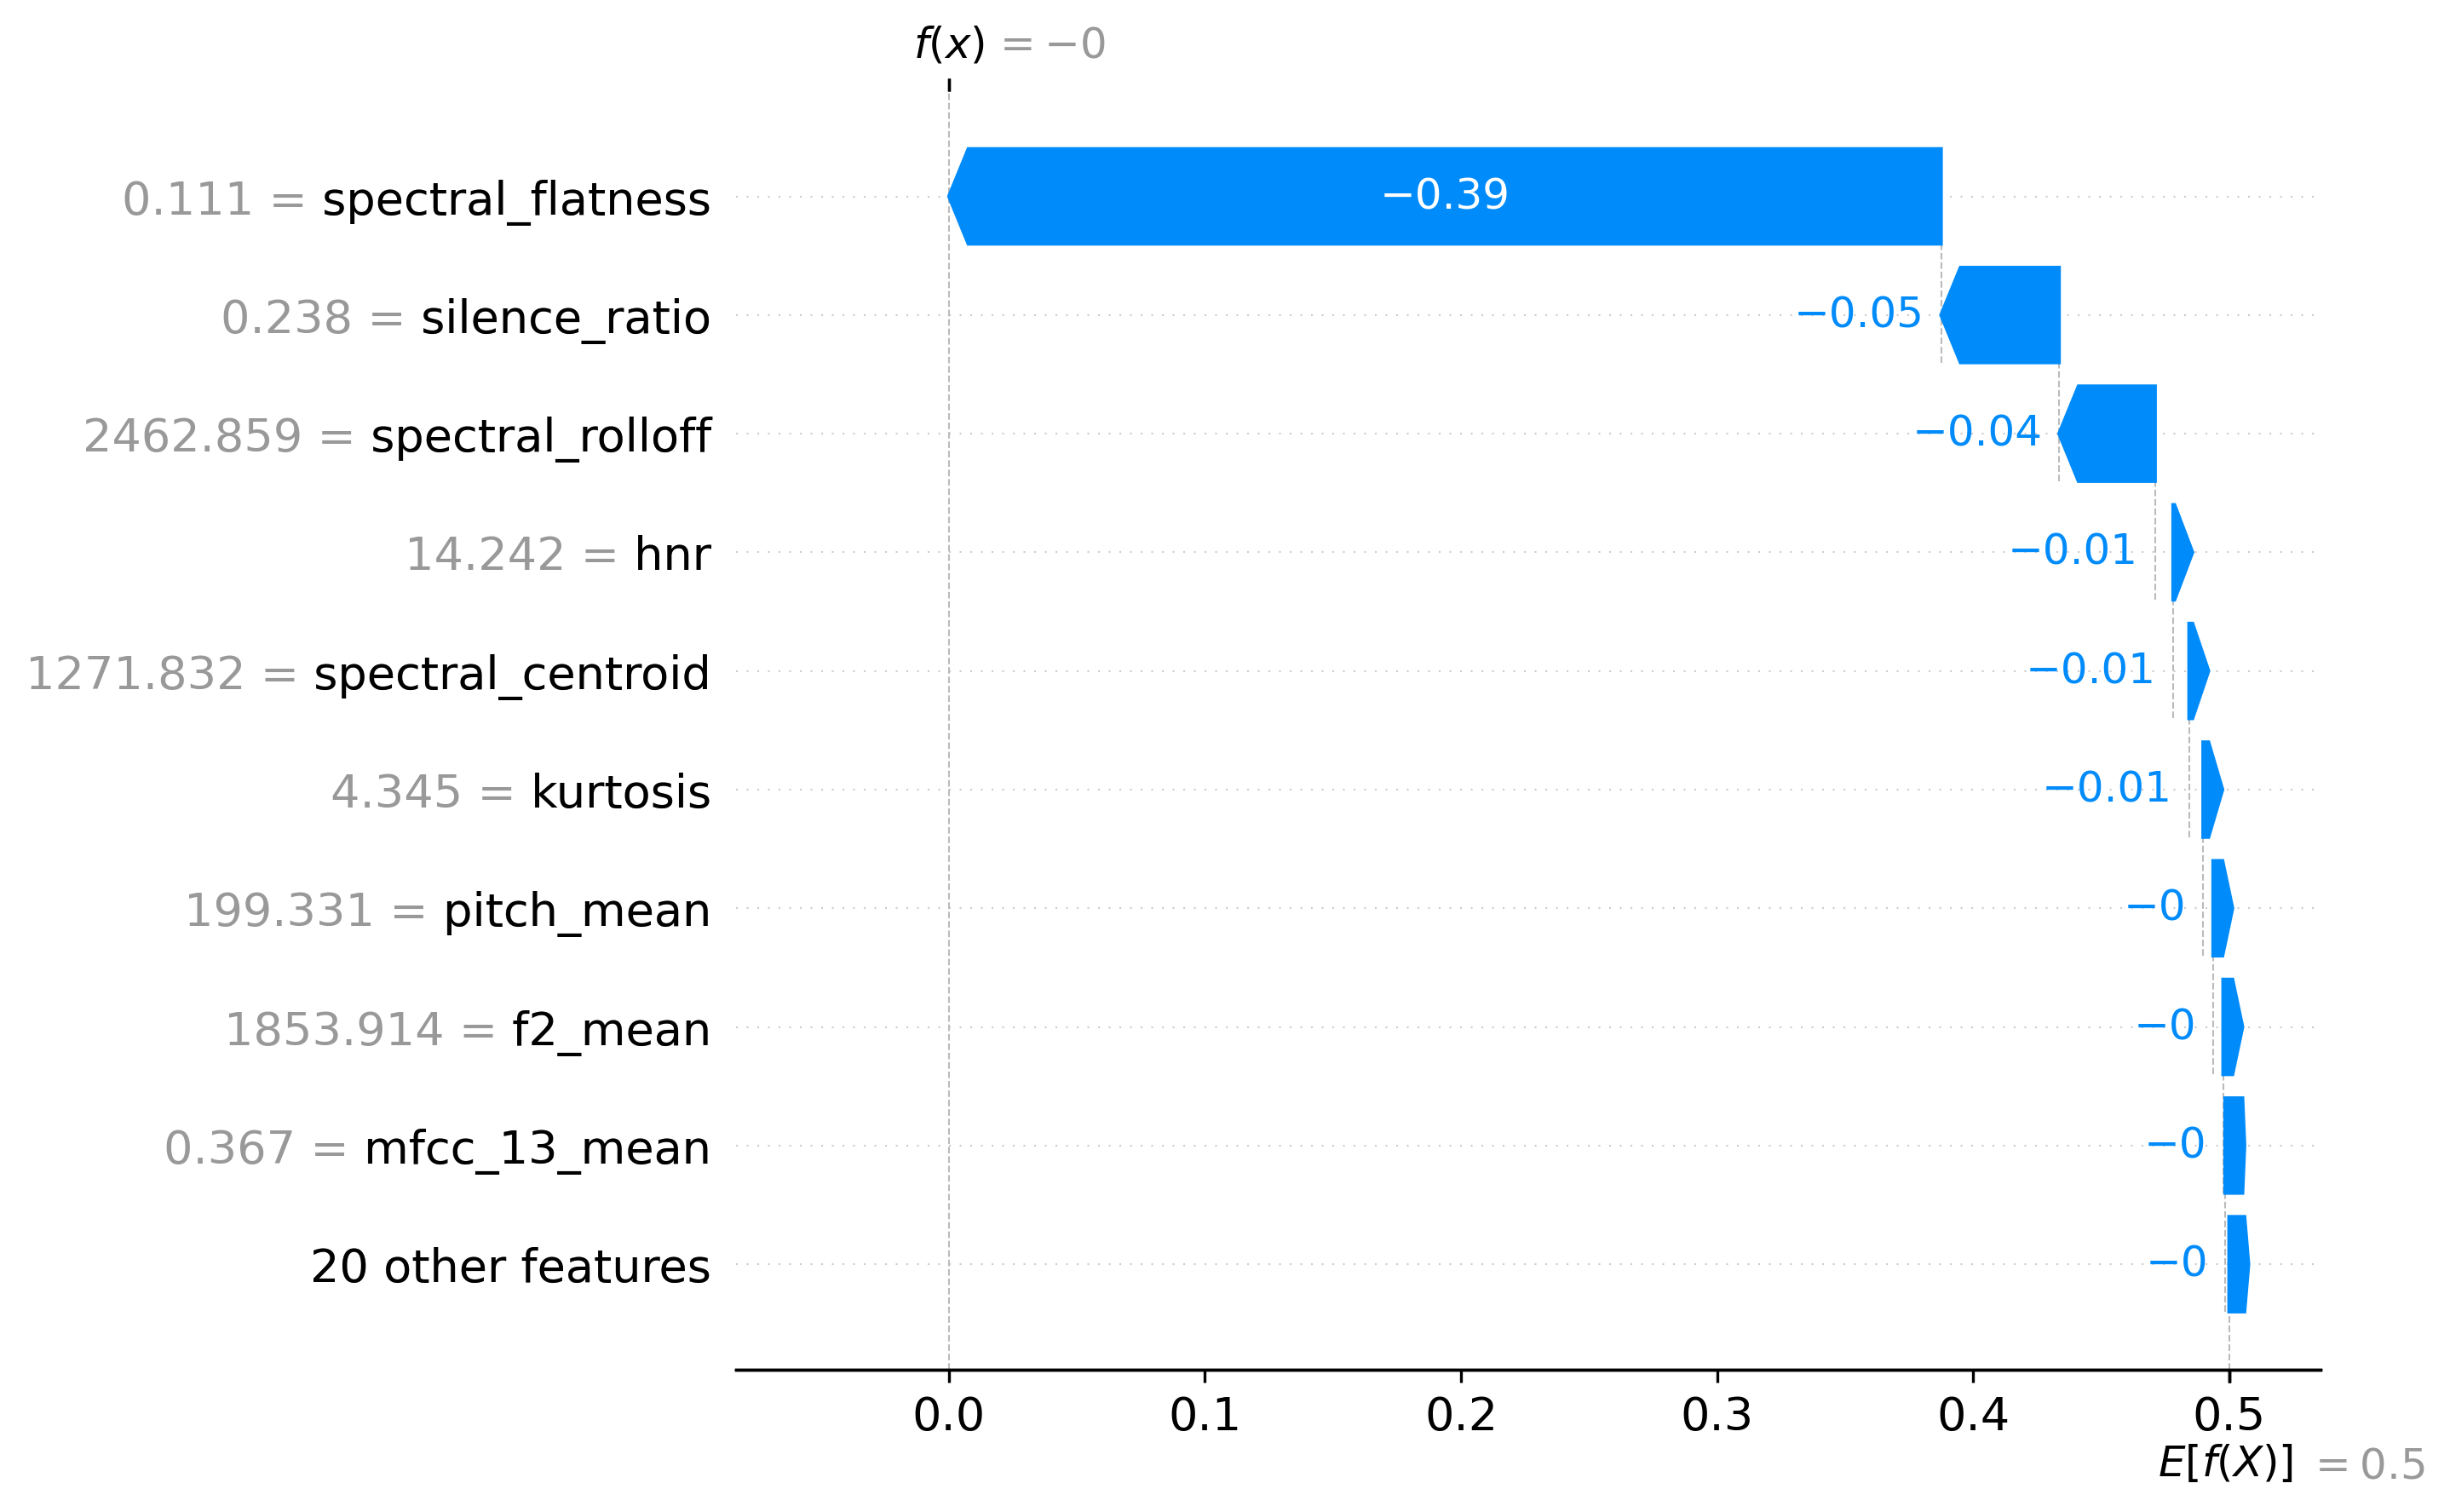
\includegraphics[width=\textwidth]{imagenes/shap_local_0.png}
		\caption{Explicación local con SHAP}
		\label{fig:shap_local}
	\end{figure}
	
\subsection*{Implementación de LIME para la interpretabilidad local del modelo}

Como complemento a SHAP, se incorporó LIME (Local Interpretable Model-agnostic Explanations) para obtener explicaciones locales de las predicciones del modelo Random Forest. LIME genera explicaciones interpretables aproximando localmente el modelo complejo mediante un modelo simple (lineal) en la vecindad de la instancia a explicar.

\subsubsection*{Funciones implementadas para explicaciones LIME}

Para integrar LIME en el flujo de trabajo, se implementó un procedimiento que permite generar explicaciones visualmente claras y personalizar su presentación para facilitar su inclusión en informes y memorias.

\paragraph{Configuración del explainer LIME}

El primer paso consiste en crear un explainer de LIME adaptado a datos tabulares:

\begin{lstlisting}[language=Python, caption=Configuración del explainer LIME]
from lime.lime_tabular import LimeTabularExplainer
import re
from IPython.display import HTML, display

# Creacion del explainer para datos tabulares
explainer = LimeTabularExplainer(
    X_train.values,                    # Datos de entrenamiento en formato numpy
    feature_names=X.columns,            # Nombres de las caracteristicas
    class_names=['label'],         # Nombres de las clases (0: Real, 1: IA)
    mode='classification'               # Modo de clasificacion
)
\end{lstlisting}

Los parámetros utilizados son:

\begin{itemize}
    \item \texttt{X\_train.values}: Matriz de características de entrenamiento en formato numpy array, necesaria para que LIME pueda muestrear la vecindad de las instancias.
    \item \texttt{feature\_names}: Lista con los nombres de las características (formantes, MFCC, etc.) para etiquetar correctamente las explicaciones.
    \item \texttt{class\_names}: Etiquetas descriptivas para las clases ('Real' y 'IA') en lugar de valores numéricos.
    \item \texttt{mode='classification'}: Indica que se trata de un problema de clasificación.
\end{itemize}

\paragraph{Generación de explicaciones para una instancia}

Para obtener la explicación de un audio específico, se utiliza el método \texttt{explain\_instance}:

\begin{lstlisting}[language=Python, caption=Generación de explicación para una instancia]
# Seleccionamos la primera instancia del conjunto de prueba como ejemplo
instancia_a_explicar = X_test.values[0]

# Generamos la explicacion
exp = explainer.explain_instance(
    instancia_a_explicar,               # Instancia a explicar
    modelo_rf.predict_proba,             # Funcion de prediccion (probabilidades)
    num_features=10                      # Numero de caracteristicas a mostrar
)
\end{lstlisting}

El método \texttt{explain\_instance} recibe:
\begin{itemize}
    \item La instancia concreta a explicar (en formato numpy array).
    \item La función de predicción del modelo (en este caso \texttt{predict\_proba}), que LIME utiliza para muestrear la vecindad y entrenar el modelo local.
    \item \texttt{num\_features}: Número de características más relevantes a incluir en la explicación (por defecto 10).
\end{itemize}

\subsubsection*{Personalización visual de las explicaciones LIME}

LIME genera por defecto visualizaciones con estilos que pueden no integrarse adecuadamente en el formato de la memoria. Para solucionarlo, se implementó un proceso de limpieza y personalización del HTML generado:

\begin{lstlisting}[language=Python, caption=Limpieza y personalización del HTML de LIME]
# Obtenemos el HTML generado por LIME
exp_html = exp.as_html()

# Removemos las etiquetas <style> internas que pueden forzar estilos no deseados
exp_html_clean = re.sub(
    r'<style.*?>.*?</style>', 
    '', 
    exp_html, 
    flags=re.DOTALL
)

# Envolvemos el HTML limpio en un contenedor con estilos personalizados
html_con_style = f"""
<style>
.lime-container * {{
    color: black !important;          # Texto en negro
    background-color: white !important; # Fondo blanco
    border-color: black !important;    # Bordes en negro
}}
</style>
<div class="lime-container">
    {exp_html_clean}
</div>
"""

# Mostramos el resultado
display(HTML(html_con_style))
\end{lstlisting}

Este proceso realiza las siguientes transformaciones:

\begin{enumerate}
    \item \textbf{Extracción del HTML}: \texttt{exp.as\_html()} genera una representación HTML completa de la explicación LIME, incluyendo estilos CSS embebidos.
    
    \item \textbf{Limpieza de estilos}: Mediante una expresión regular (\texttt{re.sub}) se eliminan todas las etiquetas \texttt{<style>} internas que LIME incluye por defecto. Esto evita conflictos con los estilos de la memoria y permite un control total sobre la apariencia.
    
    \item \textbf{Envoltura con estilos personalizados}: Se crea un contenedor \texttt{<div>} con clase \texttt{lime-container} y se definen estilos CSS que fuerzan:
    \begin{itemize}
        \item Texto en color negro (\texttt{color: black !important})
        \item Fondo blanco (\texttt{background-color: white !important})
        \item Bordes en negro (\texttt{border-color: black !important})
    \end{itemize}
    El uso de \texttt{!important} garantiza que estos estilos prevalezcan sobre cualquier otro.
    
    \item \textbf{Visualización}: Se utiliza \texttt{display(HTML(...))} de IPython para renderizar el HTML personalizado en el notebook.
\end{enumerate}

\subsubsection*{Interpretación de las explicaciones LIME}

La visualización generada por LIME muestra:

\begin{itemize}
    \item \textbf{Predicción del modelo}: La probabilidad asignada a cada clase (Real/IA) para la instancia explicada.
    
    \item \textbf{Características más influyentes}: Lista de las \texttt{num\_features} características con mayor impacto en la decisión, ordenadas por importancia.
    
    \item \textbf{Contribución de cada característica}: Barras horizontales que indican si la característica apoya la clase IA (color naranja/rojo) o la clase Real (color azul), junto con la magnitud de su contribución.
    
    \item \textbf{Valor de la característica}: Se muestra el valor concreto que tenía esa característica en el audio explicado.
\end{itemize}

\subsubsection*{Consideraciones sobre la implementación}

Durante la implementación se tuvieron en cuenta los siguientes aspectos:

\begin{itemize}
    \item \textbf{Formato de datos}: LIME requiere los datos en formato numpy array (\texttt{.values}) en lugar de DataFrame de pandas, por lo que se realiza la conversión explícita.
    
    \item \textbf{Función de predicción}: Se utiliza \texttt{predict\_proba} en lugar de \texttt{predict} para obtener las probabilidades, lo que permite a LIME capturar la confianza del modelo y no solo la clase final.
    
    \item \textbf{Número de características}: Se limitó a 8-10 características por explicación para mantener la legibilidad, aunque el parámetro es configurable.
    
    \item \textbf{Personalización visual}: La limpieza de estilos CSS garantiza que las explicaciones LIME mantengan una apariencia profesional y consistente con el resto de la memoria, evitando problemas de contraste o colores no deseados.
\end{itemize}

\subsection*{Implementación de DiCE para la generación de explicaciones contrafactuales}

Para complementar las explicaciones basadas en atribución (SHAP y LIME), se incorporó DiCE (Diverse Counterfactual Explanations) para generar explicaciones contrafactuales. DiCE responde a la pregunta: ¿qué cambios mínimos en las características de un audio clasificado como ``a'' lo harían ser clasificado como ``b'', y viceversa?

\subsubsection*{Preparación de datos para DiCE}

DiCE requiere los datos en un formato específico, combinando características y etiqueta en un mismo DataFrame:

\begin{lstlisting}[language=Python, caption=Preparación de datos para DiCE]
# Eliminacion de columnas no relevantes (ej. filename)
X_train_clean = X_train.drop(columns=['filename'], errors='ignore')
X_test_clean = X_test.drop(columns=['filename'], errors='ignore')

# Combinacion de caracteristicas con la variable objetivo
data_dice = X_train_clean.copy()
data_dice['label'] = y_train  # Variable objetivo (0: Real, 1: IA)
\end{lstlisting}

Los pasos realizados son:

\begin{itemize}
    \item \textbf{Limpieza de características no predictivas}: Se elimina la columna \texttt{filename} (si existe) ya que contiene identificadores de archivo sin valor predictivo y no tendría sentido generar contrafactuales modificándola.
    
    \item \textbf{Integración de la variable objetivo}: DiCE necesita conocer la relación entre características y etiqueta, por lo que se añade la columna \texttt{label} al DataFrame de entrenamiento.
\end{itemize}

\subsubsection*{Configuración de DiCE}

DiCE utiliza dos componentes principales: un \texttt{DataInterface} para manejar los datos y un \texttt{Model} para encapsular el clasificador:

\begin{lstlisting}[language=Python, caption=Configuración de DiCE]
import dice_ml

# Definicion del DataInterface
dice_data = dice_ml.Data(
    dataframe=data_dice,                              # DataFrame con features + target
    continuous_features=X_train_clean.columns.tolist(), # Todas las features son continuas
    outcome_name='label'                               # Nombre de la variable objetivo
)

# Encapsulacion del modelo
dice_model = dice_ml.Model(
    model=modelo_rf,        # Modelo Random Forest entrenado
    backend='sklearn'       # Backend para modelos scikit-learn
)

# Creacion del explicador DiCE
exp = dice_ml.Dice(
    dice_data,              # DataInterface
    dice_model,             # Model encapsulado
    method="random"          # Metodo de generacion ("random" o "genetic")
)
\end{lstlisting}

Los parámetros utilizados son:

\begin{itemize}
    \item \textbf{dataframe}: DataFrame completo que contiene tanto las características como la variable objetivo para el entrenamiento.
    
    \item \textbf{continuous\_features}: Lista de nombres de todas las características continuas. En este caso, todas las características de audio (formantes, MFCC, etc.) son continuas.
    
    \item \textbf{outcome\_name}: Nombre de la columna que contiene la variable objetivo ('label').
    
    \item \textbf{backend='sklearn'}: Indica que el modelo es de scikit-learn, permitiendo a DiCE acceder a los métodos necesarios.
    
    \item \textbf{method="random"}: Método de generación de contrafactuales. "random" es más rápido; también existe "genetic" para búsquedas más exhaustivas.
\end{itemize}

\subsubsection*{Generación de contrafactuales para una instancia}

Una vez configurado DiCE, se genera un conjunto de contrafactuales para una instancia específica:

\begin{lstlisting}[language=Python, caption=Generación de contrafactuales]
# Seleccion de la instancia a explicar (primera del conjunto de prueba)
query = X_test_clean.iloc[[0]]  # Usamos iloc para mantener estructura DataFrame

# Generacion de contrafactuales
e1 = exp.generate_counterfactuals(
    query_instances=query,      # Instancia(s) a explicar
    total_CFs=3,                 # Numero de contrafactuales a generar
    desired_class="opposite"     # Clase deseada (opuesta a la prediccion original)
)

# Visualizacion de resultados
e1.visualize_as_dataframe(show_only_changes=True)
\end{lstlisting}

Los parámetros de generación son:

\begin{itemize}
    \item \textbf{query\_instances}: DataFrame con una o más instancias para las que generar contrafactuales. Se utiliza \texttt{iloc[[0]]} para mantener la estructura de DataFrame (a diferencia de \texttt{iloc[0]} que devolvería una Serie).
    
    \item \textbf{total\_CFs}: Número de contrafactuales a generar (en este caso 3), permitiendo explorar diferentes alternativas para cambiar la clasificación.
    
    \item \textbf{desired\_class}: Clase objetivo para los contrafactuales. \texttt{"opposite"} indica la clase contraria a la predicción original. También se puede especificar directamente \texttt{0} (Real) o \texttt{1} (IA).
    
    \item \textbf{show\_only\_changes=True}: En la visualización, muestra únicamente las características que cambian respecto a la instancia original, facilitando la identificación rápida de las modificaciones necesarias.
\end{itemize}

\subsubsection*{Interpretación de los contrafactuales generados}

La visualización generada por \texttt{visualize\_as\_dataframe(show\_only\_changes=True)} muestra:

\begin{itemize}
    \item \textbf{Instancia original}: Valores de las características para el audio consultado y su clasificación original.
    
    \item \textbf{Contrafactuales}: Para cada uno de los \texttt{total\_CFs} generados:
    \begin{itemize}
        \item Valores de las características que cambian respecto al original (si \texttt{show\_only\_changes=True}).
        \item La nueva clasificación resultante (clase deseada).
        \item La magnitud del cambio necesario en cada característica.
    \end{itemize}
    
    \item \textbf{Diversidad}: DiCE genera contrafactuales diversos, mostrando diferentes formas de lograr el mismo cambio de clasificación (por ejemplo, modificando diferentes combinaciones de formantes o MFCC).
\end{itemize}

La salida para la primera instancia es:

\subsubsection*{Interpretación en el contexto de detección de deepfakes}

Las explicaciones contrafactuales permiten responder preguntas como:

\begin{itemize}
    \item \textbf{Para un audio clasificado como IA}: "¿Qué características acústicas deberían cambiar para que el modelo lo considere voz real, y en qué magnitud?"
    
    \item \textbf{Para un audio clasificado como real}: "¿Qué modificaciones lo harían ser clasificado como generado por IA?"
    
    \item \textbf{Vías alternativas}: DiCE muestra múltiples formas de lograr el cambio, revelando si hay ``caminos'' principales (modificar ciertos formantes) o alternativos (modificar MFCC específicos).
\end{itemize}

\subsubsection*{Consideraciones sobre la implementación}

Durante la implementación se tuvieron en cuenta los siguientes aspectos:

\begin{itemize}
    \item \textbf{Eliminación de columnas no relevantes}: Características como 'filename' se eliminan porque no tienen sentido en un contrafactual (no se puede modificar el nombre del archivo para cambiar la clasificación).
    
    \item \textbf{Selección de instancia}: Se utiliza \texttt{iloc[[index]]} en lugar de \texttt{iloc[index]} para mantener la estructura de DataFrame requerida por DiCE.
    
    \item \textbf{Método de generación}: Se eligió \texttt{method=random} por su eficiencia computacional, aunque para análisis más exhaustivos se puede utilizar \texttt{method=genetic}.
    
    \item \textbf{Visualización enfocada}: El parámetro \texttt{show\_only\_changes=True} facilita la interpretación al mostrar únicamente las características que realmente cambian, evitando abrumar con información redundante.
    
    \item \textbf{Clase deseada}: El valor \texttt{opposite} es útil cuando se quiere explorar el cambio de clase, pero también se puede especificar explícitamente \texttt{0} o \texttt{1} si se busca una dirección concreta.
\end{itemize}